\documentclass{beamer}
\usepackage{polski}
\usepackage[utf8]{inputenc}
\usepackage{graphics}
\usepackage{minted}
\usepackage{fvextra}
\usepackage{caption}
\usepackage{epigraph}
\usepackage{array}
\newcolumntype{L}[1]{>{\raggedright\let\newline\\\arraybackslash\hspace{0pt}}m{#1}}
\newcolumntype{C}[1]{>{\centering\let\newline\\\arraybackslash\hspace{0pt}}m{#1}}
\newcolumntype{R}[1]{>{\raggedleft\let\newline\\\arraybackslash\hspace{0pt}}m{#1}}
\definecolor{NiceGreen}{RGB}{40,200,0}
\definecolor{CoolDarkGray}{RGB}{50,50,50}


\title{\texttt{Projekt aplikacji do ekstremalnego uczenia maszynowego do klasyfikacji big data}}
\author{Ahmed Abdelkarim, Aleksandra Hernik}

\begin{document}
\setbeamercolor{background canvas}{bg=CoolDarkGray}
\setbeamercolor{title}{fg=NiceGreen}
\setbeamercolor{frametitle}{fg=NiceGreen}
\setbeamercolor{structure}{fg=white}
\setbeamertemplate{section in toc}{%
    \textcolor{NiceGreen}{\inserttocsectionnumber)}   \inserttocsection \par}

\addtobeamertemplate{navigation symbols}{}{%
    \usebeamerfont{footline}%
    \usebeamercolor[fg]{footline}%
    \hspace{1em}%
    \insertframenumber/\inserttotalframenumber
}

\setbeamercolor{normal text}{fg=white}\usebeamercolor*{normal text}
\begin{frame}
  \maketitle
\end{frame}

\begin{frame}{Plan}
  \tableofcontents[currentsection]
\end{frame}

\section{Czym jest ELM?}
\begin{frame}{Klasyfikacja}
\begin{figure}
	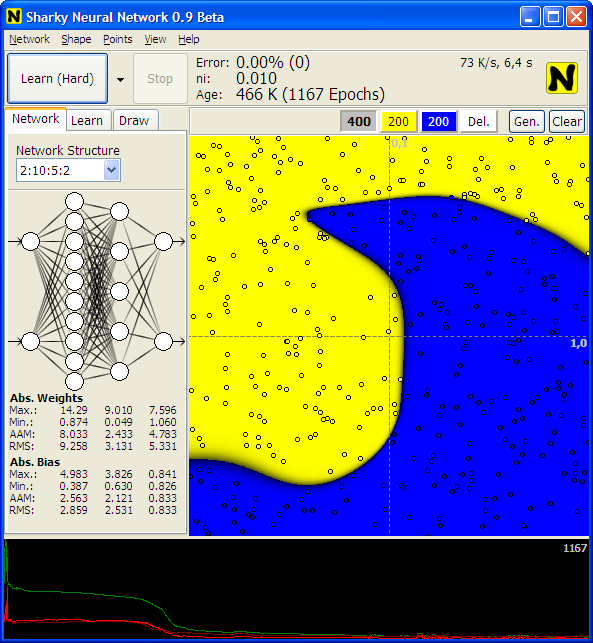
\includegraphics[scale=0.3]{klasyfikacja.png}
\end{figure}
\end{frame}
\begin{frame}{Czym jest ELM?}
ELM to sieć neuronowa, spełniająca proste założenia:
\begin{itemize}
\item jest jednowarstwowa,
\item jest jednokierunkowa,
\item wagi wejściowe są losowane,
\item trening polega na wyznaczeniu wag wyjściowych,
\item wyznaczanie wag wyjściowych to operacja liniowa.
\end{itemize}
\end{frame}
\begin{frame}{Schemat ELM}
\begin{figure}[H]
\centering
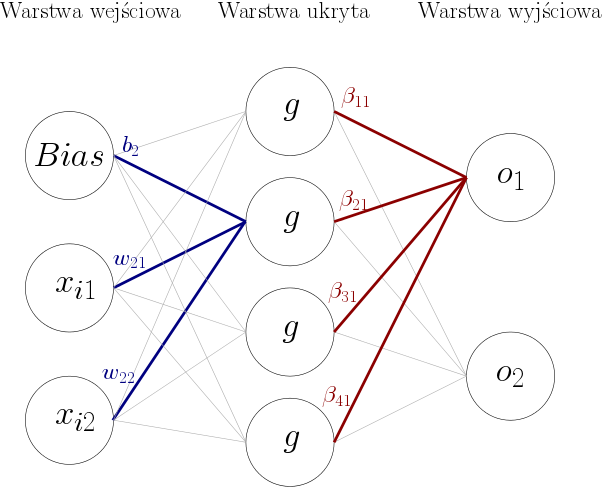
\includegraphics[width=0.8\textwidth]{schemat_sieci.png}
\caption{Schemat SLFN typu ELM}
\end{figure}
\end{frame}
\begin{frame}{Dlaczego ELM?}
Jeśli wierzyć autorom dotychczasowych prac:
\begin{itemize}
\item szybsze nawet 1 000 000 razy od tradycyjnych metod,
\item mimo tego, osiągają dobre wyniki.
\end{itemize}
\begin{figure}[H]
\centering
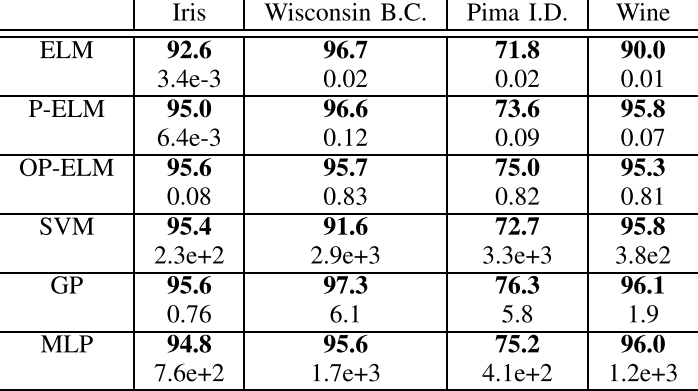
\includegraphics[width=0.85\textwidth]{obiecywane_rezultaty.png}
\caption{Rezultaty obiecywane przez Antona Akusoka}
\end{figure}
\end{frame}
\section{Cel pracy}
\begin{frame}{Cele projektu}
\begin{itemize}
\item Uruchomienie algorytmu na testach różnych rozmiarów
\item Zmierzenie czasu trwania uczenia
\item Przetestowanie jakości uczenia
\item Porównanie aplikacji w Pythonie i Matlabie
\item Rozważenie możliwych ulepszeń algorytmu
\end{itemize}
\end{frame}
\section{Implementacja}
\begin{frame}{Przykładowe dane testowe}
Znaleziony zestaw danych wykorzystany w konkursie uczenia maszynowego w 2014:
\begin{itemize}
\item Kilkadziesiąt zmierzonych cech lasów w USA
\item Elewacja, nachylenie, odległość od wody i wiele innych
\item Wynik: dominujący gatunek drzew (jeden z siedmiu)
\end{itemize}
\end{frame}
\begin{frame}{Zadania}
\begin{itemize}
\item Obudowanie istniejącego kodu klasami, ułatwiającymi puszczanie testów i zbieranie informacji
\item Znalezienie danych testowych
\item Uruchomienie testów i analiza wyników
\item[?] Wprowadzenie własnych funkcji wyliczających błąd 
\item[?] Przetestowanie innych funkcji aktywacji
\end{itemize}
\end{frame}

\begin{frame}{Diagram klas}
\begin{figure}
	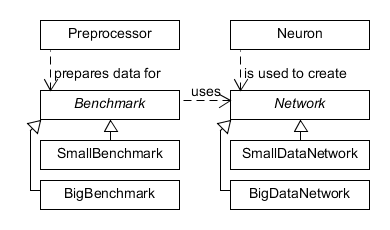
\includegraphics[width=\textwidth]{classescompact.png}
\end{figure}
\end{frame}


\begin{frame}{Harmonogram}
\begin{table}[H]
\begin{tabular}{| L{6cm} |c|c|}
\hline
\textbf{Etap} & \textbf{Początek} & \textbf{Koniec} \\

\hline
Przygotowanie pierwszego rozdziału dokumentacji & 10.10.2016 & 02.11.2016 \\
\hline
Opracowanie modelu pracy sieci ELM & 17.10.2016 & 30.10.2016 \\
\hline
Analiza narzędzi &  31.10.2016 & 06.11.2016 \\
\hline
Projekt techniczny &  07.11.2016 & 13.11.2016 \\
\hline
Implementacja i napisanie drugiego rozdziału pracy & 07.11.2016 & 11.12.2016 \\
\hline
Tworzenie, wykonywanie i opisanie testów & 12.12.2016 & 18.12.2016 \\
\hline
Instrukcja użytkownika & 19.12.2016 & 20.12.2016 \\
\hline
\end{tabular}
\end{table}
\end{frame}
\begin{frame}{Źródła}
\begin{thebibliography}{9}
\bibitem{akusok-hpelm}
  A. Akusok, K.-M. Björk, Y. Miche, A. Lendasse,
  \emph{High-Performance Extreme Learning Machines: A Complete Toolbox for Big Data Applications}
\bibitem{huang-elm-tap:ta}
  A. G.-B. Huang, L. Chen, C.-K. Siew, 
  \emph{Extreme Learning Machine: Theory and Applications}
\bibitem{dane}
	Dane dotyczące klasyfikacji lasów: https://www.kaggle.com/c/forest-cover-type-prediction
\end{thebibliography}
\end{frame}

\end{document}

\endinput